\documentclass[a4paper,ngerman,landscape,12pt]{scrartcl}

\usepackage[utf8]{inputenc}

\usepackage[ngerman]{babel}
\usepackage{hyperref}

\usepackage{graphicx}

\usepackage[protrusion=true,expansion=true]{microtype}

\usepackage{lmodern}
\usepackage{tabto}
\usepackage{multicol}

\usepackage[normalem]{ulem}

\setlength\parskip{\medskipamount}
\setlength\parindent{0pt}

\usepackage{geometry}
\geometry{tmargin=0.2cm,bmargin=0.0cm,lmargin=0.75cm,rmargin=0.75cm}

\pagestyle{empty}

\begin{document}

\begin{center}
  \Huge
  \textbf{\sf Pizzaseminar in den Ferien?}

  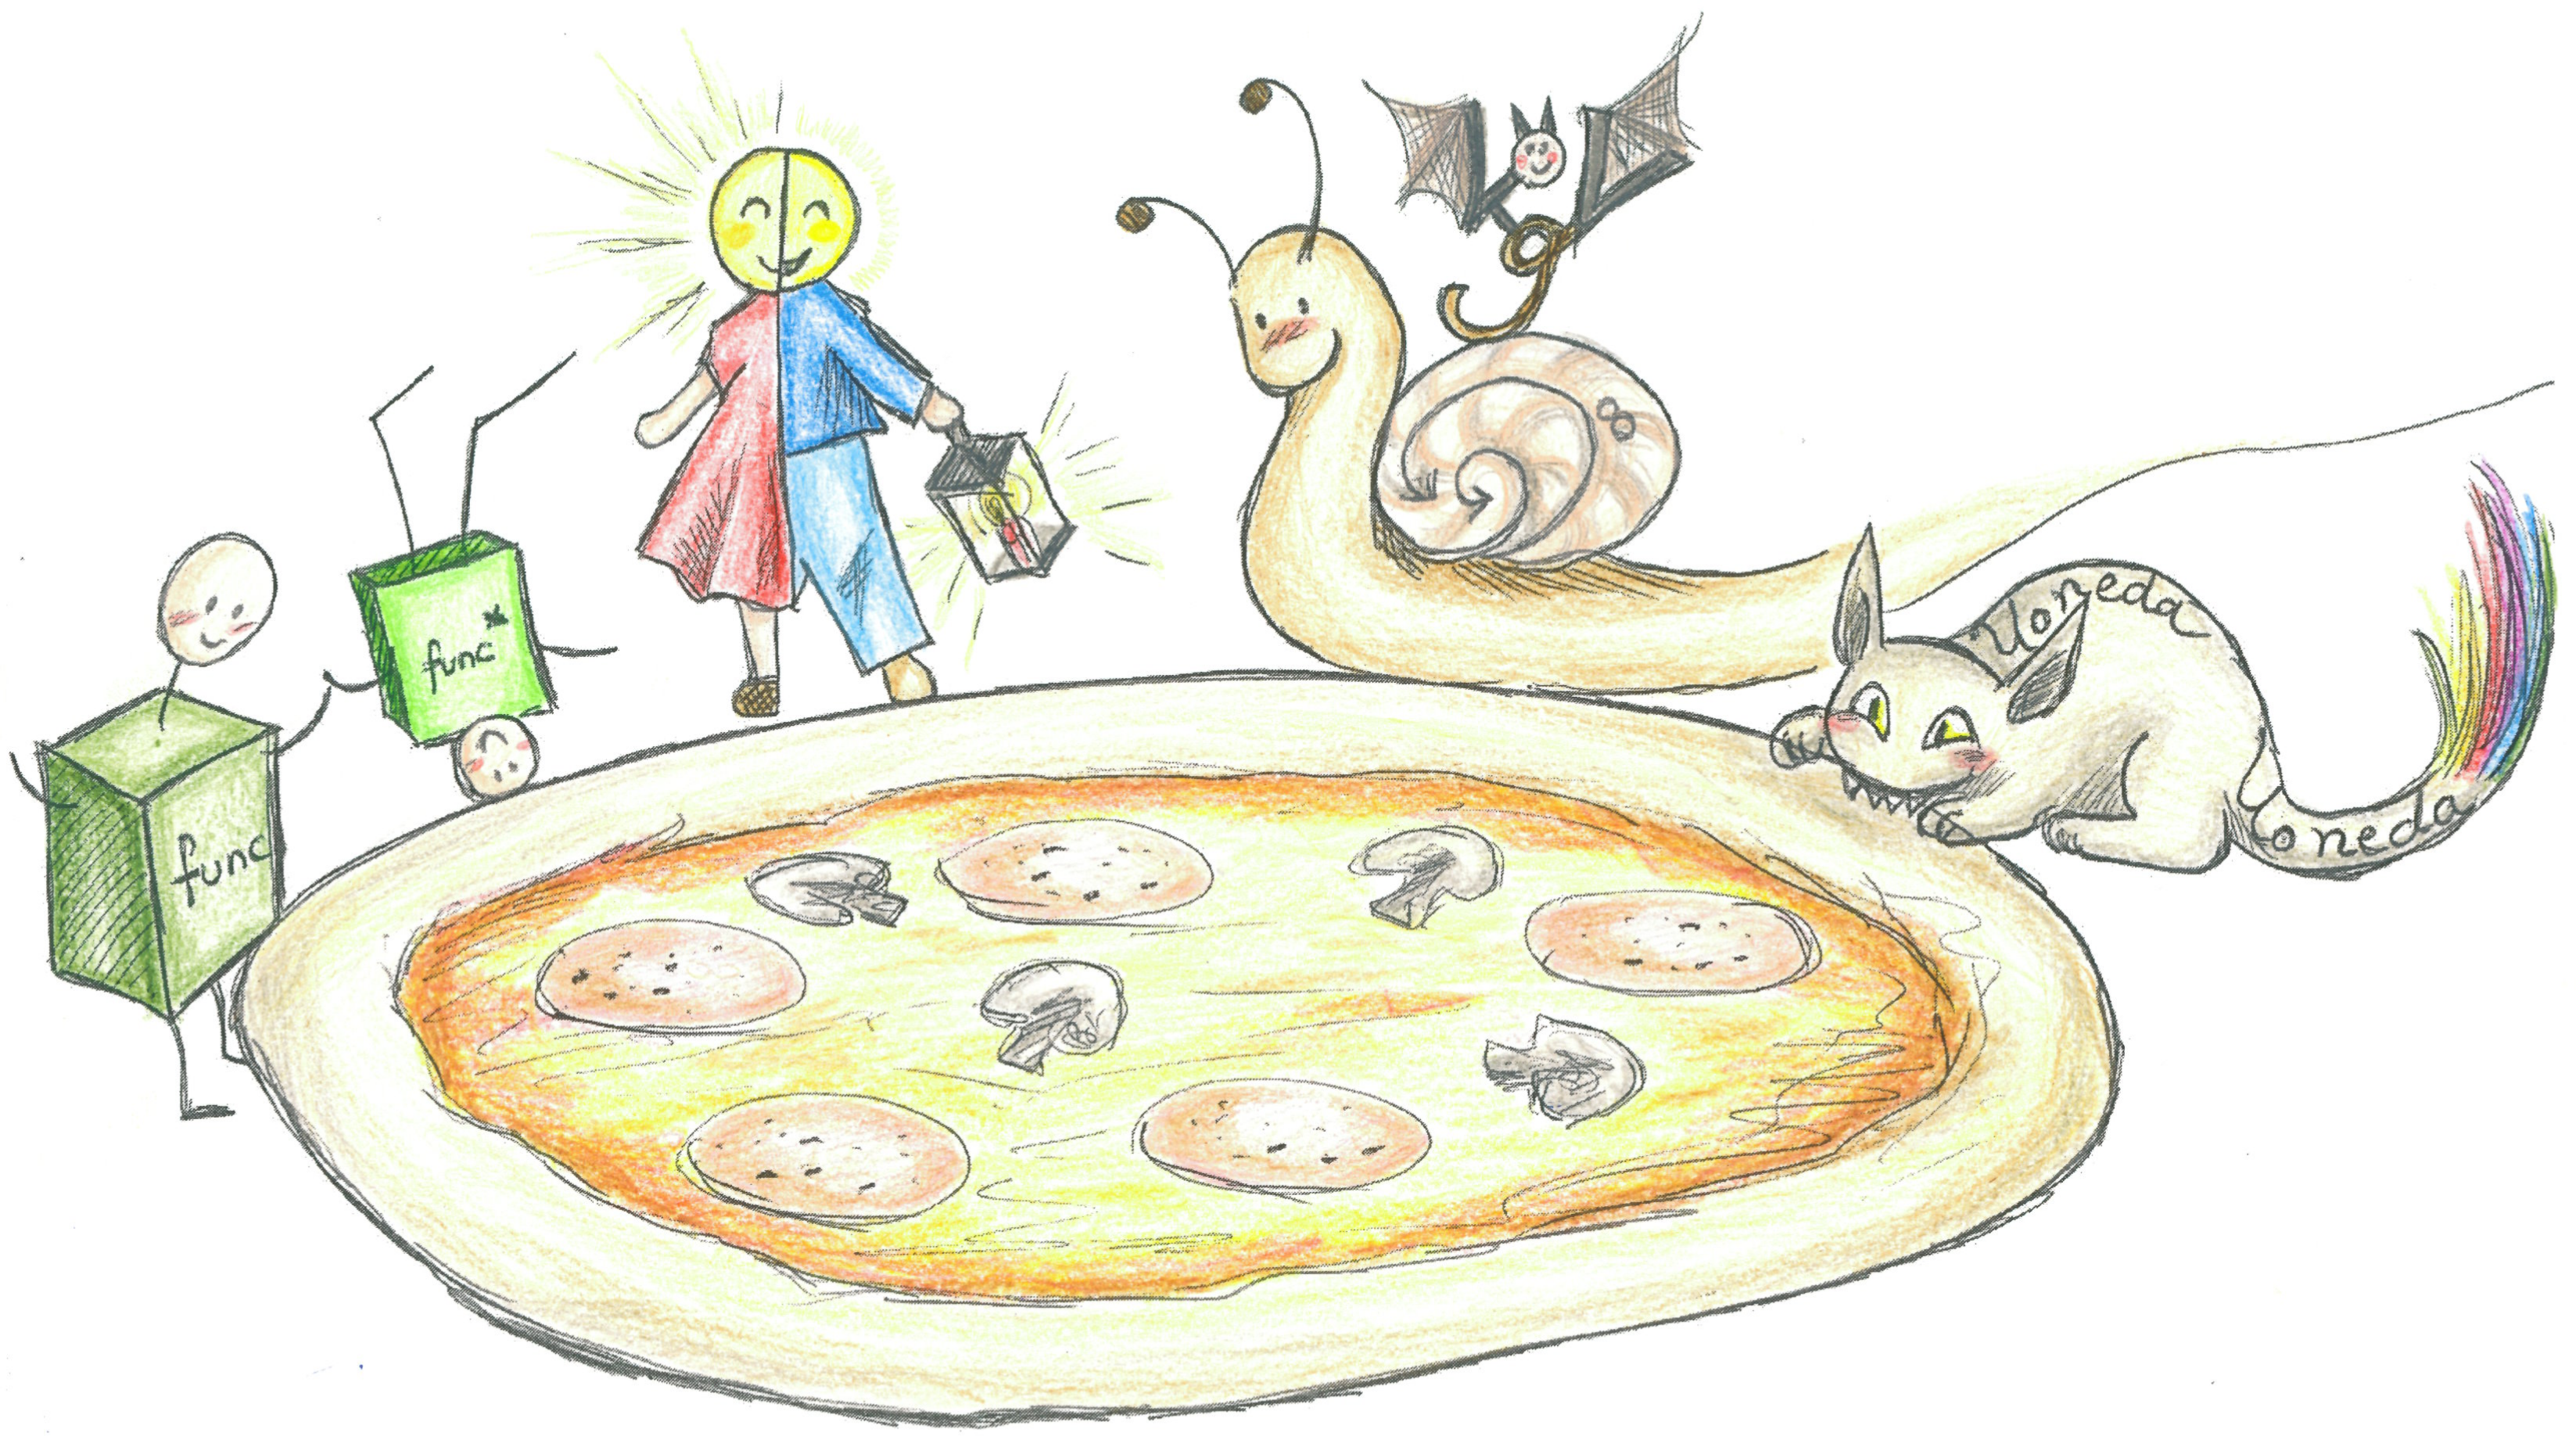
\includegraphics[scale=0.83]{pizza-farbig-hq}

  \vfill
  \large
  \begin{minipage}{1.00\textwidth}
    \setlength\parskip{\medskipamount}
    \setlength\columnsep{1.5cm}
    \begin{multicols*}{2}
Ein Pizzaseminar ist ein Seminar von Studenten für Studenten über
interessante Themen der Mathematik. Der Name rührt daher, weil man bei den
Treffen Pizza bestellen kann; inhaltlich kann man etwa die Gelegenheit nutzen,
um sich gemeinsam ein Thema zu erarbeiten oder über
Abschlussarbeiten zu berichten.

Zum ersten Mal gab es das Pizzaseminar in den letzten \mbox{Ferien}: Da haben wir uns
die Grundlagen von Kategorien\-theorie angeeignet und dann einige Anwendungen
gesehen, siehe \url{http://pizzaseminar.speicherleck.de/} für ein Skript und
weitere Materialien.

\columnbreak

Wer Interesse hat, aktiv oder passiv an einer hypothetischen Zweitauflage des
Pizzaseminars mitzumachen, kann sich völlig unverbindlich bei Ingo Blechschmidt
melden (Büro~2031/L1 oder \url{iblech@web.de}), idealerweise unter Angabe
möglicher Zeiträume.

In erster Näherung sind nur Vorkenntnisse aus
LA~I/Algebra~I und Ana~I erforderlich, Erstsemester sind also explizit
willkommen! Neben dem fachlichen Nutzen kann man Erfahrung für offizielle
Seminarvorträge sammeln, mit Leistungspunkten sollte man aber nicht rechnen.
\end{multicols*}
\newpage
  \end{minipage}

  \begin{minipage}{1.00\textwidth}
    Themenvorschläge:
    \begin{itemize}
      \item Tausendundeine Umformulierungen der riemannschen Vermutung
      \item Anwendungen der Hauptkomponentenanalyse in Statistik und Numerik
      \item Eine Parabel über einen König, einen Philosophen und den Stein der
      Weisen: \\ konstruktive Mathematik und algorithmischer Inhalt klassischer
      Mathematik
      \item Mathematische Modellierung natürlicher Sprache durch kategoriellen
      Schnickschnack
      \item Zombie-Apokalypse~$3_1$ -- Rückkehr der gordischen Unknoten
      \item \sout{Rechnen mit konkreten Zahlenwerten}
    \end{itemize}
  \end{minipage}
\end{center}

% Inhalte/inhaltlich

\end{document}
